\subsection{Helioviewer}\label{ssec:hv}

SunPy provides the ability to download images hosted by the
Helioviewer Project (\href{http://helioviewer.org}{http://helioviewer.org}).  
The aim of the Helioviewer Project is to enable
the exploration of solar and heliospheric data from multiple data
sources (such as instrumentation and feature/event catalogues) via
easy-to-use visual interfaces. The Helioviewer Project have developed two client 
applications that allow users to browse images and create movies of the Sun taken 
by a variety of instruments: \href{http://www.helioviewer.org}{Helioviewer.org}, a 
Google Maps-like web application, and \href{http://www.jhelioviewer.org}{JHelioviewer}, 
a movie streaming desktop application. In order to manage all of this data, the Helioviewer
project maintains archives of all of its data in JPEG2000 format (for further
details on the Helioviewer Project see \cite{muller2009}). The
JPEG2000 files are typically highly compressed compared to the source
FITS files they are generated from but high-fidelity, and thus can be used to quickly
visualise large amounts of data from multiple sources.  SunPy is
also used in Helioviewer production servers to manage the download and
ingestion of JPEG2000 files from remote servers.

The Helioviewer Project categorises image data based on the physical
construction of the source instrument, using a simple hierarchy:
observatory $\rightarrow$ instrument $\rightarrow$ detector
$\rightarrow$ measurement, where '$\rightarrow$' means 'provides
(possibly multiple)'.  
%schriste - say what?!
Each Helioviewer Project JPEG2000 file contains
metadata which are based (in part) on the original FITS header
information, and carry sufficient information to permit overlay with
other Helioviewer JPEG2000 files. Images can be accessed either as
PNGs (Section \ref{sssec:hv:png}) or as JPEG2000 files (Section
\ref{sssec:hv:jp}).

\subsubsection{Download a PNG file}\label{sssec:hv:png}

The Helioviewer API allows composition and overlay of images from
multiple sources, based on the positioning metadata in the source FITS
file.  SunPy accesses this overlay/composition capability through the
\texttt{download\_png} method of the Helioviewer client.  Listing
\ref{code:hv:overlaid} gives an example of the composition of three
separate image layers in to a single image.

\begin{listing}[H]
\begin{minted}[bgcolor=bg]{pycon}
>>> from sunpy.net.helioviewer import HelioviewerClient
>>> hv = HelioviewerClient()
>>> hv.download_png('2099/01/01', 6,
...                 "[SDO,AIA,AIA,304,1,100],[SDO,AIA,AIA,193,1,50],"+
...                 "[SOHO,LASCO,C2,white-light,1,100]",
...                 x0=0, y0=0, width=768, height=768)
\end{minted}
\begin{center}
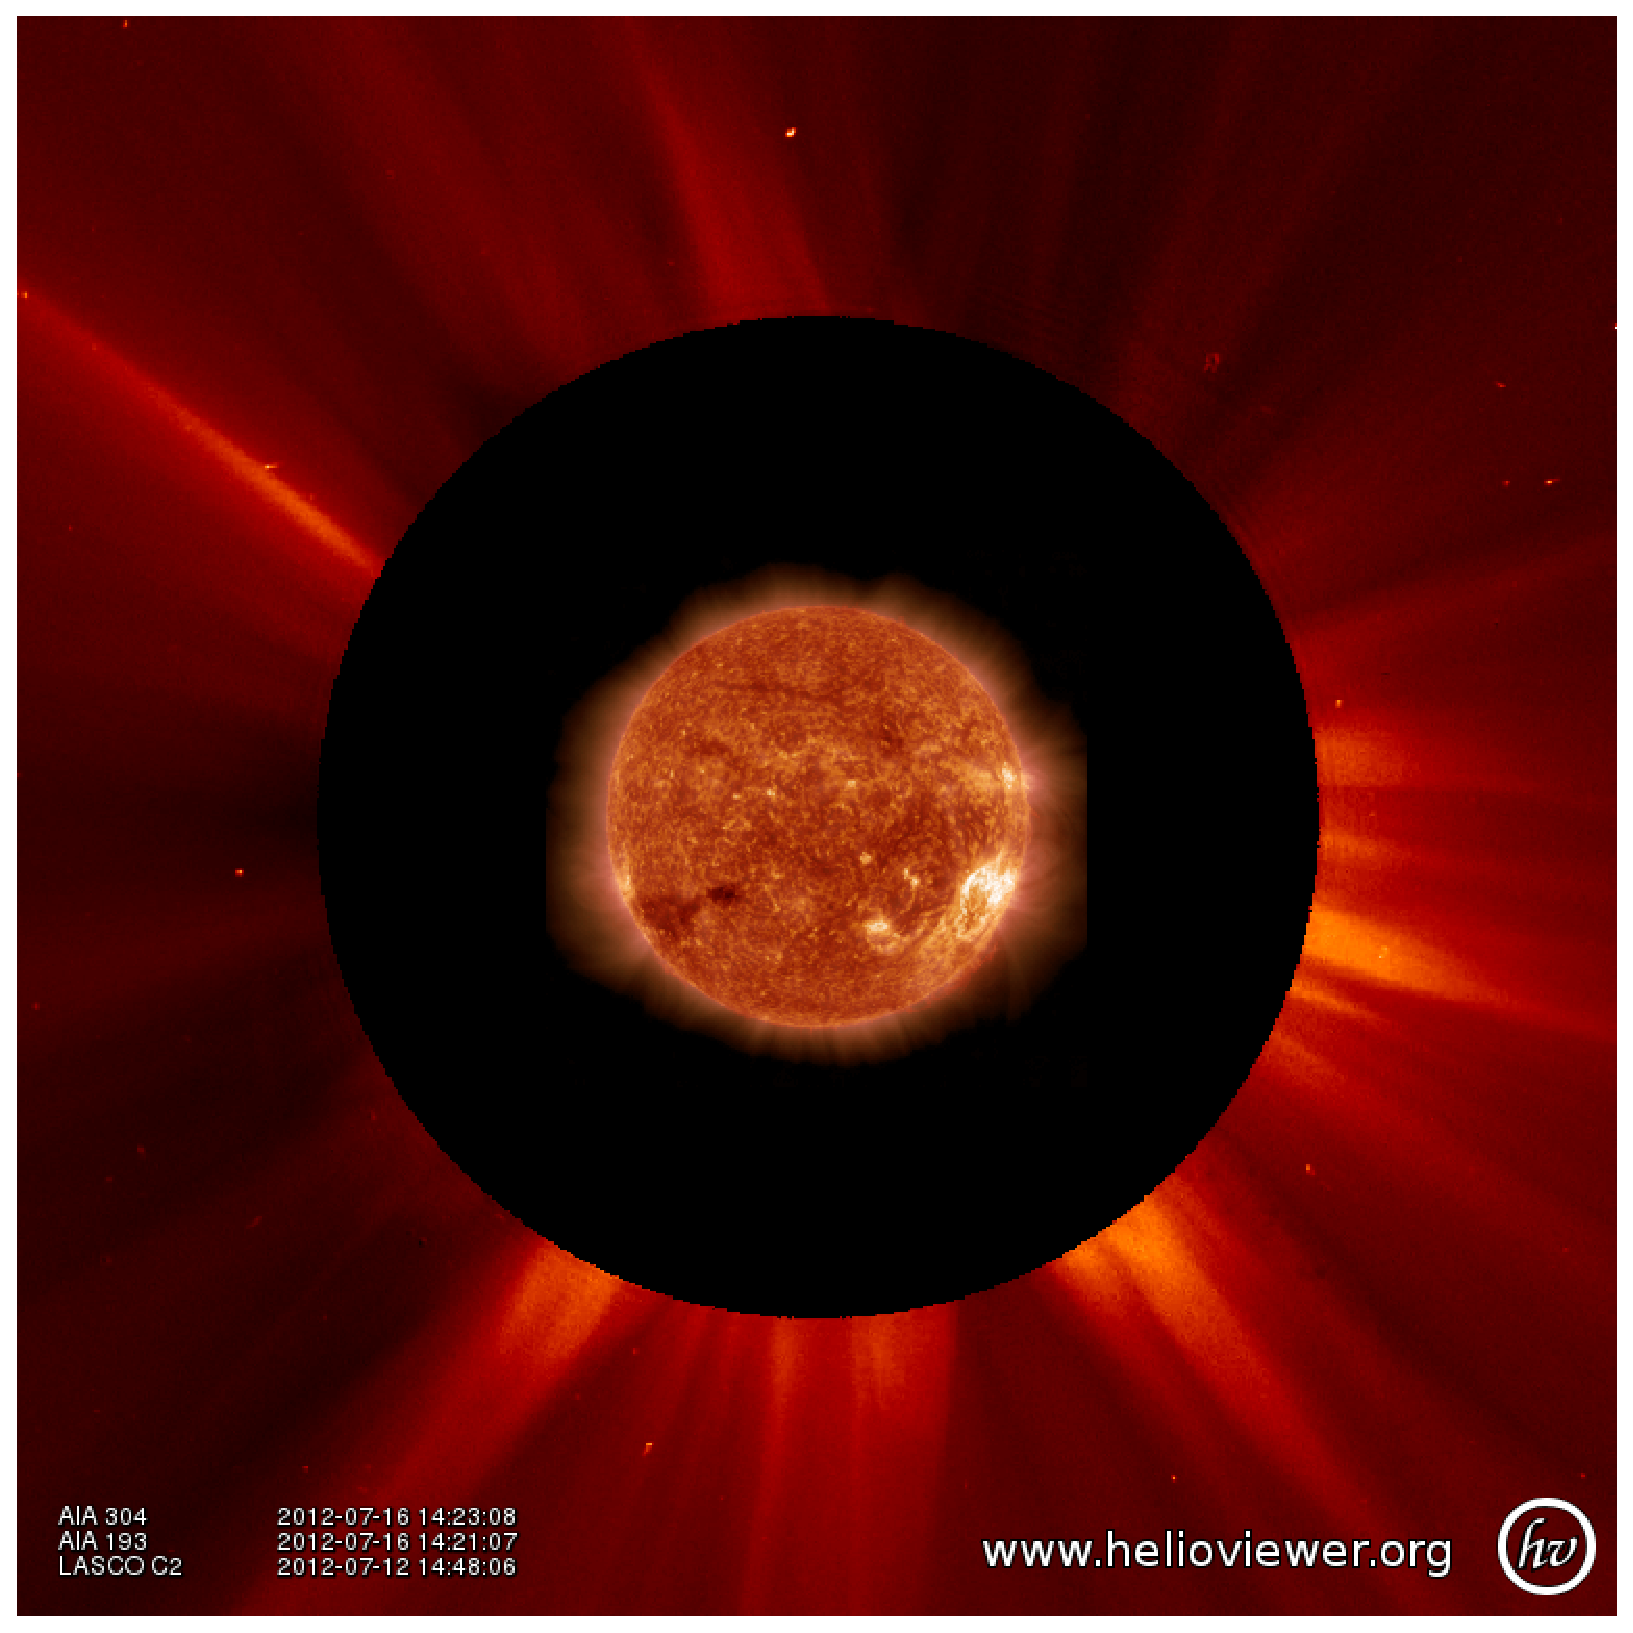
\includegraphics[width=0.6\columnwidth]{helioviewer_overlay_example}
\end{center}
\caption{Acquisition of a PNG image composed from data from three
  separate sources.}
\label{code:hv:overlaid}
\end{listing}

The first argument is the requested time of the image.  Helioviewer
selects images closest to the requested time.  In this case, the
requested time is in the future and so Helioviewer will find the most
recent available images from each source.  The second argument refers
to the image resolution in arcseconds per pixel (larger values mean
lower resolution).  The third argument is a comma-delimited string of
the three requested image layers, the details of which are enclosed
in parentheses. The image layers are described using the observatory
$\rightarrow$ instrument $\rightarrow$ detector $\rightarrow$
measurement combination described above, along with the final two
numbers that denote the visibility and the opacity of the image layer
respectively (1/0 is visible/invisible with opacity in the range
$0\rightarrow100$, with $100$ meaning fully opaque).  The quantities
\texttt{x0} and \texttt{y0} are the $x$ and $y$ centre points about
which to centre the image (measured in helio-projective cartesian
coordinates), and the \texttt{width} and \texttt{height} are the pixel
values for the image dimensions.

This functionality makes it simple for SunPy users to generate complex
images from multiple, correctly overlaid, image data sources.

\subsubsection{Download a JPEG2000 file}\label{sssec:hv:jp}

As noted above, Helioviewer JPEG2000 files contain metadata that allow
positioning of the image data.  There is sufficient metadata in each
file to permit the creation of a SunPy \texttt{Map} object (see Section
\ref{ssec:map}) from a Helioviewer JPEG2000 file.  This allows image
data to be manipulated in the same way as any other map object.

Reading JPEG2000 file into a SunPy session requires installing two
other pieces of software. The first, 
\href{http://www.openjpeg.org}{\texttt{OpenJPEG}}, is an open
source library for reading and writing JPEG2000 files.  The other package 
required is 
\href{https://github.com/quintusdias/glymur}{\texttt{glymur}}, an
interface between Python and the OpenJPEG libraries (note that these
packages are {\it not} required to use the functionality described in
Section \ref{sssec:hv:png}).

Listing \ref{code:downloadjp2} demonstrates the querying, downloading,
reading and conversion of a Helioviewer JPEG2000 file into a SunPy map
object.  This functionality allows users to visualise and manipulate
Helioviewer-supplied image data in an identical fashion to a SunPy \texttt{Map}
object generated from FITS data (see Section \ref{ssec:map}).

\begin{listing}[H]
\begin{minted}[bgcolor=bg]{pycon}
>>> import sunpy.map
>>> filepath = hv.download_jp2('2012/07/05 00:30:00',
...                            observatory='SDO',
...                            instrument='HMI', detector='HMI', 
...                            measurement='continuum')
>>> sunpy.map.Map(filepath).submap([200,550],[-400,-200]).peek()
\end{minted}
\begin{center}
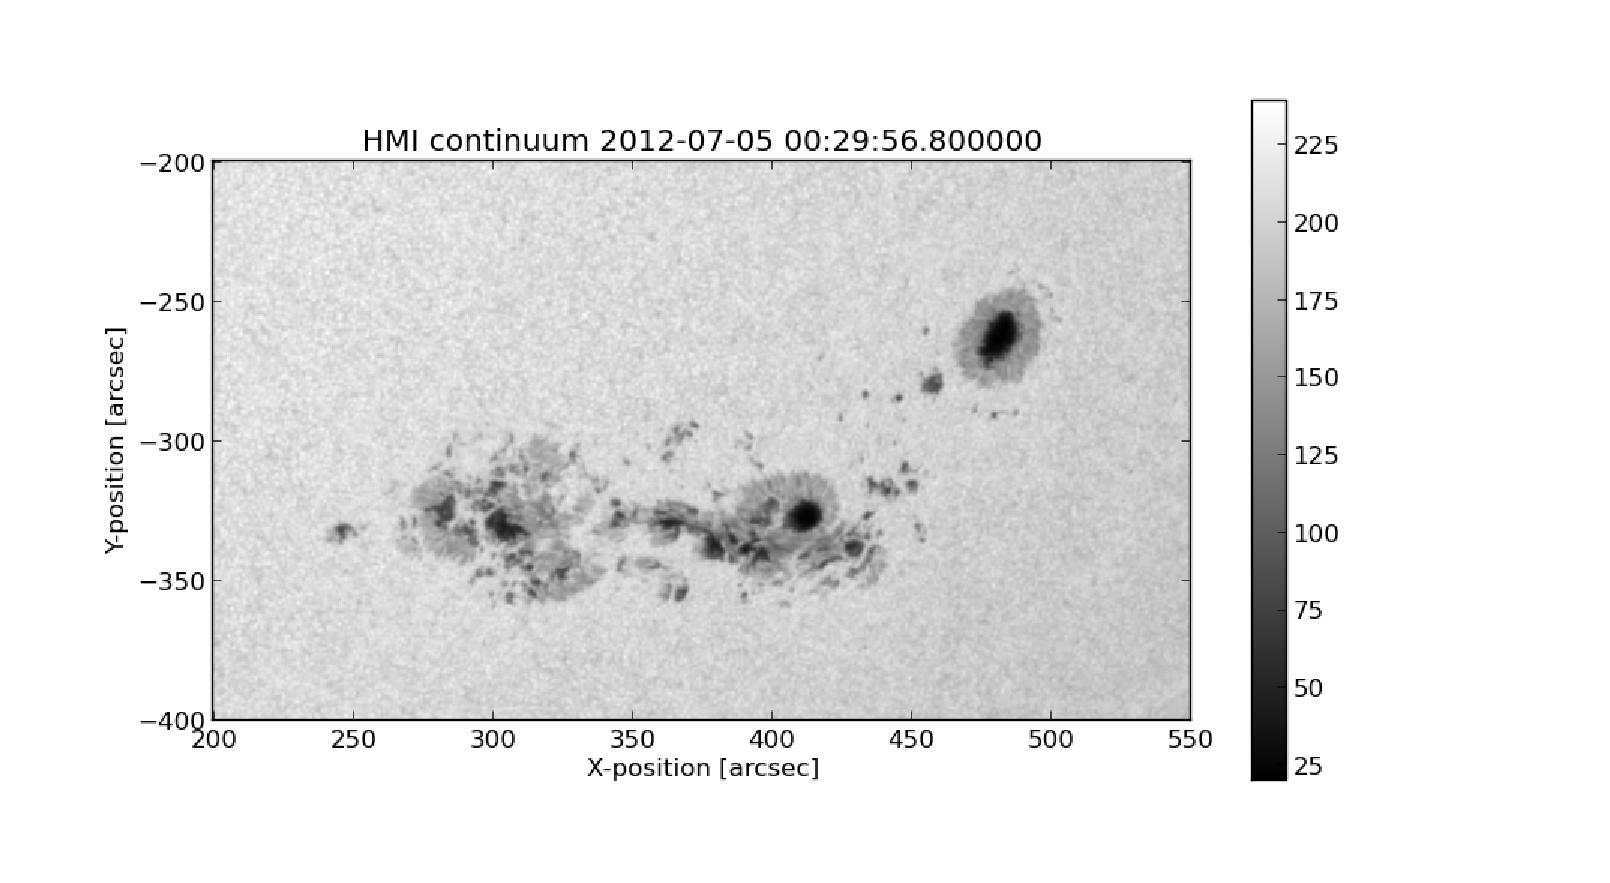
\includegraphics[width=0.8\columnwidth]{helioviewer_hmi_continuum_jp2_to_map}
\end{center}
\caption{Acquisition and display of a Helioviewer JPEG2000 file as a
  SunPy \texttt{Map} object.}
\label{code:downloadjp2}
\end{listing}
